\begin{apendicesenv}
\partapendices

\chapter{CINTIL}
\label{ap_cintil}

\section{Tabelas}
\label{ap_cintil_tab}

\begin{center}
    \begin{longtable}{|p{0.4\textwidth}|p{0.1\textwidth}|p{0.1\textwidth}|p{0.1\textwidth}|p{0.1\textwidth}|p{0.1\textwidth}|}
\caption{Tabela com resultados completos do CINTIL}\\
\hline
 & \textbf{LP} & \textbf{LR} & \textbf{F1} & \textbf{Exact} & \textbf{N} \\
\hline
\endfirsthead
\multicolumn{6}{c}%
{\tablename\ \thetable\ -- \textit{Continuação da página anterior}} \\
\hline
 & \textbf{LP} & \textbf{LR} & \textbf{F1} & \textbf{Exact} & \textbf{N} \\
\hline
\endhead
\hline \multicolumn{6}{r}{\textit{Continua na próxima página}} \\
\endfoot
\hline
\endlastfoot
    % \csvautotabular{tabelas/resultados-cintil_testes.csv}
    1 & 	 & 	 & 	 & 	 & 		\\
    pcfg LP/LR summary evalb: &  58.09  &  65.99  &  61.79  &  27.46  &  863\\
    dep DA summary evalb:  &  69.47  &  69.47  &  69.47  &  34.26  &  858\\
    factor LP/LR summary evalb:  &  59.69  &  68.88  &  63.96  &  28.38  &  863\\
    factor Tag summary evalb:  &  81.94  &  82.78  &  82.36  &  54.92  &  863\\
    2 & 	 & 	 & 	 & 	 & 	\\
    pcfg LP/LR summary evalb:  &  62.52  &  62.32  &  62.42  &  18.27  &  93\\
    dep DA summary evalb:  &  70.69  &  70.69  &  70.69  &  24.73  &  93\\
    factor LP/LR summary evalb:  &  67.82  &  69.88  &  68.83  &  20.43  &  93\\
    factor Tag summary evalb:  &  85.89  &  86.35  &  86.12  &  38.7  &  93\\
    3 & 	 & 	 & 	 & 	 & 	\\
    pcfg LP/LR summary evalb:  &  55.69  &  54.58  &  55.13  &  15.0  &  100\\
    dep DA summary evalb:  &  67.4  &  67.4  &  67.4  &  24.0  &  100\\
    factor LP/LR summary evalb:  &  64.95  &  65.75  &  65.35  &  25.0  &  100\\
    factor Tag summary evalb:  &  83.63  &  83.96  &  83.79  &  36.0  &  100\\
    4 & 	 & 	 & 	 & 	 & 	\\
    pcfg LP/LR summary evalb:  &  54.03  &  51.31  &  52.63  &  13.79  &  87\\
    dep DA summary evalb:  &  70.44  &  70.44  &  70.44  &  29.88  &  87\\
    factor LP/LR summary evalb:  &  61.23  &  59.49  &  60.35  &  12.64  &  87\\
    factor Tag summary evalb:  &  85.37  &  85.37  &  85.37  &  35.63  &  87\\
    5 & 	 & 	 & 	 & 	 & 	\\
    pcfg LP/LR summary evalb:  &  61.48  &  64.64  &  63.02  &  23.17  &  82\\
    dep DA summary evalb:  &  63.81  &  63.81  &  63.81  &  24.39  &  82\\
    factor LP/LR summary evalb:  &  64.61  &  69.12  &  66.79  &  30.48  &  82\\
    factor Tag summary evalb:  &  84.94  &  84.94  &  84.94  &  40.24  &  82\\
    6 & 	 & 	 & 	 & 	 & 	\\
    pcfg LP/LR summary evalb:  &  58.81  &  57.61  &  58.21  &  14.49  &  69\\
    dep DA summary evalb:  &  69.88  &  69.88  &  69.88  &  27.53  &  69\\
    factor LP/LR summary evalb:  &  68.56  &  68.06  &  68.31  &  20.28  &  69\\
    factor Tag summary evalb:  &  85.97  &  86.35  &  86.16  &  36.23  &  69\\
    7 & 	 & 	 & 	 & 	 & 	\\
    pcfg LP/LR summary evalb:  &  62.51  &  63.67  &  63.09  &  25.33  &  75\\
    dep DA summary evalb:  &  74.13  &  74.13  &  74.13  &  36.0  &  75\\
    factor LP/LR summary evalb:  &  67.72  &  69.08  &  68.4  &  28.0  &  75\\
    factor Tag summary evalb:  &  88.09  &  88.09  &  88.09  &  44.0  &  75\\
    8 & 	 & 	 & 	 & 	 & 	\\
    pcfg LP/LR summary evalb:  &  53.03  &  54.05  &  53.54  &  16.41  &  67\\
    dep DA summary evalb:  &  68.04  &  68.04  &  68.04  &  26.86  &  67\\
    factor LP/LR summary evalb:  &  59.23  &  61.76  &  60.47  &  17.91  &  67\\
    factor Tag summary evalb:  &  85.65  &  85.65  &  85.65  &  35.82  &  67\\
    9 & 	 & 	 & 	 & 	 & 	\\
    pcfg LP/LR summary evalb:  &  61.76  &  57.5  &  59.56  &  21.11  &  90\\
    dep DA summary evalb:  &  67.12  &  67.12  &  67.12  &  26.96  &  89\\
    factor LP/LR summary evalb:  &  65.31  &  62.84  &  64.05  &  24.44  &  90\\
    factor Tag summary evalb:  &  86.35  &  86.35  &  86.35  &  45.55  &  90\\
    10 & 	 & 	 & 	 & 	 & 	\\
    pcfg LP/LR summary evalb:  &  63.32  &  63.98  &  63.65  &  20.89  &  67\\
    dep DA summary evalb:  &  65.9  &  65.9  &  65.9  &  28.35  &  67\\
    factor LP/LR summary evalb:  &  65.13  &  67.55  &  66.32  &  19.4  &  67\\
    factor Tag summary evalb:  &  84.63  &  85.01  &  84.82  &  40.29  &  67
    \label{tab:cintil_result_full}
\end{longtable}
    % 1 &  &  &  &  & \\
    % pcfg LP/LR summary evalb: & 45.43 & 45.04 & 45.24 & 11.23 & 730\\
    % dep DA summary evalb: & 57.22 & 57.22 & 57.22 & 18.24 & 729\\
    % factor LP/LR summary evalb: & 51.83 & 52.56 & 52.19 & 13.56 & 730\\
    % factor Tag summary evalb: & 74.71 & 74.87 & 74.79 & 18.76 & 730\\
    % 2 &  &  &  &  & \\
    % pcfg LP/LR summary evalb: & 42.87 & 46.27 & 44.5 & 4.26 & 1500\\
    % dep DA summary evalb: & 49.18 & 49.18 & 49.18 & 14.77 & 1448\\
    % factor LP/LR summary evalb: & 42.89 & 47.23 & 44.96 & 4.06 & 1500\\
    % factor Tag summary evalb: & 67.1 & 67.48 & 67.29 & 4.13 & 1500\\
    % 3 &  &  &  &  & \\
    % pcfg LP/LR summary evalb: & 39.8 & 42.86 & 41.27 & 3.54 & 1493\\
    % dep DA summary evalb: & 49.28 & 49.28 & 49.28 & 11.84 & 1478\\
    % factor LP/LR summary evalb: & 39.97 & 44.02 & 41.9 & 3.68 & 1493\\
    % factor Tag summary evalb: & 62.74 & 63.1 & 62.92 & 3.61 & 1493\\
    % 4 &  &  &  &  & \\
    % pcfg LP/LR summary evalb: & 43.55 & 47.44 & 45.42 & 4.18 & 1506\\
    % dep DA summary evalb: & 59.71 & 59.71 & 59.71 & 17.44 & 1364\\
    % factor LP/LR summary evalb: & 43.76 & 48.13 & 45.84 & 4.38 & 1506\\
    % factor Tag summary evalb: & 64.98 & 65.38 & 65.18 & 4.24 & 1506\\
    % 5 &  &  &  &  & \\
    % pcfg LP/LR summary evalb: & 41.82 & 43.7 & 42.74 & 4.1 & 1511\\
    % dep DA summary evalb: & 46.98 & 46.98 & 46.98 & 15.76 & 1484\\
    % factor LP/LR summary evalb: & 41.57 & 45.19 & 43.3 & 4.3 & 1511\\
    % factor Tag summary evalb: & 63.41 & 63.79 & 63.6 & 4.16 & 1511\\
    % 6 &  &  &  &  & \\
    % pcfg LP/LR summary evalb: & 41.24 & 43.26 & 42.23 & 3.47 & 1524\\
    % dep DA summary evalb: & 53.29 & 53.29 & 53.29 & 15.39 & 1507\\
    % factor LP/LR summary evalb: & 41.68 & 44.69 & 43.14 & 3.74 & 1524\\
    % factor Tag summary evalb: & 61.77 & 62.12 & 61.95 & 3.34 & 1524\\
    % 7 &  &  &  &  & \\
    % pcfg LP/LR summary evalb: & 44.51 & 45.43 & 44.97 & 6.65 & 1518\\
    % dep DA summary evalb: & 47.55 & 47.55 & 47.55 & 12.83 & 1449\\
    % factor LP/LR summary evalb: & 44.15 & 46.29 & 45.19 & 6.85 & 1518\\
    % factor Tag summary evalb: & 61.98 & 62.35 & 62.17 & 5.73 & 1518\\
    % 8 &  &  &  &  & \\
    % pcfg LP/LR summary evalb: & 41.61 & 44.06 & 42.8 & 4.71 & 1526\\
    % dep DA summary evalb: & 51.59 & 51.59 & 51.59 & 12.51 & 1494\\
    % factor LP/LR summary evalb: & 42.01 & 44.93 & 43.42 & 4.65 & 1526\\
    % factor Tag summary evalb: & 62.75 & 63.13 & 62.94 & 5.5 & 1526\\
    % 9 &  &  &  &  & \\
    % pcfg LP/LR summary evalb: & 38.85 & 44.39 & 41.43 & 3.12 & 1503\\
    % dep DA summary evalb: & 51.94 & 51.94 & 51.94 & 12.97 & 1464\\
    % factor LP/LR summary evalb: & 38.82 & 45.17 & 41.76 & 2.99 & 1503\\
    % factor Tag summary evalb: & 64.52 & 64.91 & 64.72 & 3.79 & 1503\\
    % 10 &  &  &  &  & \\
    % pcfg LP/LR summary evalb: & 39.92 & 44.13 & 41.92 & 2.88 & 1526\\
    % dep DA summary evalb: & 50.25 & 50.25 & 50.25 & 10.94 & 1325\\
    % factor LP/LR summary evalb: & 39.06 & 44 & 41.38 & 2.81 & 1526\\
    % factor Tag summary evalb: & 61.49 & 61.84 & 61.67 & 2.03 & 1526

% \begin{table}[h]
%     \centering
%     % \begin{tabular}{c|c}
%     %      &  \\
%     %      & 
%     % \end{tabular}
%     \csvautotabular{tabelas/resultados-cintil_testes.csv}
%     \caption{Tabela com resultados completos do CINTIL}
%     \label{tab:cintil_result_full}
% \end{table}
\end{center}

\section{Imagens}
\label{ap_cintil_imagens}

\section{Códigos}
\label{ap_cintil_codigos}

O \textit{parsing} do PS é feito executando o comando \ref{lst:cod_parsing_cintil}.
\begin{center}
    \begin{lstlisting}[breaklines, caption={Execução de \textit{parsing} em sentenças transduzidas a partir do CINTIL},label={lst:cod_parsing_cintil},language=Bash]
    java -cp stanford-parser.jar -mx4g edu.stanford.nlp.parser.lexparser.LexicalizedParser -loadFromSerializedFile ~/<diretorio de armazenamento>/serialGrammarBOSQUE1 sentencas_teste_cintil.txt
\end{lstlisting}
\end{center}

Explicando rapidamente na Tabela \ref{tab:tab_exec_basico_cintil}.

\begin{center}
    \begin{table}[h!]
    \centering
    \begin{tabular}{p{0.8\textwidth}}
        \begin{itemize}
            \item [-cp] \textit{ClassPath}. Indica o diretório onde se encontra a classe principal a ser executada
            \item [-mx4g] Quantidade de memória usada. No caso, 4 GB.
            \item [LexicalizedParser] \textit{Parser} utilizado, dentre os disponibilizados
            \item [-loadFromSerializedFile] Carrega a gramática serializada, gerada na execução de treinamento anterior
            \item [arquivo.txt] Arquivo que contém sentenças a serem classificadas pelo SP
            % \item [-outputFilesDirectory] Define o diretório onde os arquivos de saída serão escritos. 
            % \item [-testTreebank] Diretório onde se encontra o treebank a ser usado para teste. Os números no formato $a-b$ indicam o primeiro e o último arquivo, respectivamente. Números no formato $a-b,c-d$ indicam dois blocos de arquivos. Atente para não usar o mesmo bloco dos treinos, ou o parser passará por \textit{overfitting}, e terá resultados enviesados.
        \end{itemize}
    \end{tabular}
    \caption[Comandos para uma execução simples do \textit{Stanford Parser}]{Comandos para uma execução simples do \textit{Stanford Parser}, utilizando o terminal.}
    \label{tab:tab_exec_basico_cintil}
\end{table}
\end{center}
% --------------------------------------------------------------------
\chapter{BOSQUE}
\label{ap_bosque}

\section{Tabelas}
\label{ap_bosque_tab}

\begin{center}
    \begin{longtable}{|p{0.4\textwidth}|p{0.1\textwidth}|p{0.1\textwidth}|p{0.1\textwidth}|p{0.1\textwidth}|p{0.1\textwidth}|}
\caption{Tabela com resultados completos do BOSQUE}\\
\hline
 & \textbf{LP} & \textbf{LR} & \textbf{F1} & \textbf{Exact} & \textbf{N} \\
\hline
\endfirsthead
\multicolumn{6}{c}%
{\tablename\ \thetable\ -- \textit{Continuação da página anterior}} \\
\hline
 & \textbf{LP} & \textbf{LR} & \textbf{F1} & \textbf{Exact} & \textbf{N} \\
\hline
\endhead
\hline \multicolumn{6}{r}{\textit{Continua na próxima página}} \\
\endfoot
\hline
\endlastfoot
    1 &  & &  &  & \\
    pcfg LP/LR summary evalb & 44.6 & 41.62 & 43.06 & 6.82 & 3650\\
    dep DA summary evalb & 68.39 & 68.39 & 68.39 & 14.04 & 3646\\
    factor LP/LR summary evalb & 47.31 & 45.97 & 46.63 & 8.73 & 3650\\
    factor Tag summary evalb & 64.63 & 66.08 & 65.35 & 9.28 & 3650\\
    2 &  &  &  &  & \\
    pcfg LP/LR summary evalb & 43.75 & 40.77 & 42.21 & 6.95 & 3652\\
    dep DA summary evalb & 67.26 & 67.26 & 67.26 & 12.92 & 3651\\
    factor LP/LR summary evalb & 46.41 & 45.27 & 45.83 & 8.13 & 3652\\
    factor Tag summary evalb & 64.24 & 65.68 & 64.96 & 9.44 & 3652\\
    3 &  &  &  &  & \\
    pcfg LP/LR summary evalb & 44.15 & 41.48 & 42.78 & 8.5 & 3657\\
    dep DA summary evalb & 67.66 & 67.66 & 67.66 & 13.26 & 3650\\
    factor LP/LR summary evalb & 46.92 & 45.92 & 46.42 & 8.28 & 3657\\
    factor Tag summary evalb & 64.18 & 65.59 & 64.88 & 8.12 & 3657\\
    4 &  &  &  &  & \\
    pcfg LP/LR summary evalb & 44.52 & 41.4 & 42.9 & 7.64 & 3661\\
    dep DA summary evalb & 67.7 & 67.7 & 67.7 & 13.34 & 3657\\
    factor LP/LR summary evalb & 46.21 & 44.64 & 45.41 & 8.44 & 3661\\
    factor Tag summary evalb & 63.95 & 65.36 & 64.65 & 9.09 & 3661\\
    5 &  &  &  &  & \\
    pcfg LP/LR summary evalb & 44.17 & 41.56 & 42.82 & 8.5 & 3667\\
    dep DA summary evalb & 67.17 & 67.17 & 67.17 & 13.62 & 3663\\
    factor LP/LR summary evalb & 46.16 & 45.11 & 45.63 & 8.75 & 3667\\
    factor Tag summary evalb & 63.76 & 65.16 & 64.45 & 8.8 & 3667\\
    6 &  &  &  &  & \\
    pcfg LP/LR summary evalb & 44.29 & 41.02 & 42.59 & 7.54 & 3656\\
    dep DA summary evalb & 67.65 & 67.65 & 67.65 & 13.54 & 3654\\
    factor LP/LR summary evalb & 47.03 & 45.46 & 46.23 & 8.2 & 3656\\
    factor Tag summary evalb & 64.05 & 65.5 & 64.77 & 8.78 & 3656\\
    7 &  &  &  &  & \\
    pcfg LP/LR summary evalb & 44.92 & 42.14 & 43.49 & 8.23 & 3654\\
    dep DA summary evalb & 67.67 & 67.67 & 67.67 & 13.11 & 3652\\
    factor LP/LR summary evalb & 46.97 & 46.05 & 46.5 & 8.83 & 3654\\
    factor Tag summary evalb & 64.62 & 66.04 & 65.32 & 9.49 & 3654\\
    8 &  &  &  &  & \\
    pcfg LP/LR summary evalb & 44.83 & 41.62 & 43.17 & 8.68 & 3663\\
    dep DA summary evalb & 68.34 & 68.34 & 68.34 & 13.95 & 3661\\
    factor LP/LR summary evalb & 46.84 & 46.13 & 46.49 & 8.4 & 3663\\
    factor Tag summary evalb & 65.08 & 66.52 & 65.79 & 10.04 & 3663\\
    9 &  &  &  &  & \\
    pcfg LP/LR summary evalb & 43.88 & 40.83 & 42.3 & 7.49 & 3658\\
    dep DA summary evalb & 67.52 & 67.52 & 67.52 & 12.94 & 3654\\
    factor LP/LR summary evalb & 45.88 & 44.69 & 45.28 & 8.25 & 3658\\
    factor Tag summary evalb & 64.06 & 65.5 & 64.77 & 9.02 & 3658\\
    10 &  &  &  &  & \\
    pcfg LP/LR summary evalb & 43.78 & 40.54 & 42.1 & 8 & 3649\\
    dep DA summary evalb & 67.49 & 67.49 & 67.49 & 12.76 & 3644\\
    factor LP/LR summary evalb & 46.64 & 45.48 & 46.05 & 9.64 & 3649\\
    factor Tag summary evalb & 63.97 & 65.43 & 64.69 & 9.78 & 3649
    \label{tab:bosque_result_full}
\end{longtable}
\end{center}

\begin{center}
    \begin{longtable}{|p{0.15\linewidth}|p{0.2\linewidth}|p{0.15\linewidth}|p{0.15\linewidth}|p{0.25\linewidth}|}
\caption{Tabela de conversão completa: BOSQUE para PTB (Funções)}\\
\hline
\textbf{Tag Original (Português)} & \textbf{Nome da Tag} & \textbf{Tag Convertida} & \textbf{Ocorrências} & \textbf{Observações}\\
\hline
\endfirsthead
\multicolumn{5}{c}%
{\tablename\ \thetable\ -- \textit{Continuação da página anterior}} \\
\hline
\textbf{Tag Original (Português)} & \textbf{Nome da Tag} & \textbf{Tag Convertida} & \textbf{Ocorrências} & \textbf{Observações} \\
\hline
\endhead
\hline \multicolumn{5}{r}{\textit{Continua na próxima página}} \\
\endfoot
\hline
\endlastfoot

    \textgreater A & dependente em adjp ou advp (antecede o núcleo) & \textgreater A & 371 & Explicado em \ref{subsec:bosque_a}\\
    A\textless  & dependente em adjp ou advp (segue o núcleo) & A\textless & 272 & Explicado em  \ref{subsec:bosque_a}\\
    A\textless ARG & Estrutura não descrita em \citeonline{freitas2007biblia} & não convertida & 12 & \\
    A\textless arg & Estrutura não descrita em  \citeonline{freitas2007biblia}  & não convertida & 45 & \\
    ACC & objecto directo (incluindo alguns tipos de se) & depende da \textit{form\_tag} & 4315 & Explicado em \ref{subsec:tag_acl}\\
    ACC-PASS & função do clítico se numa oração passiva (partícula apassivante) & NP & 39 & Refere-se ao uso de pronomes clíticos numa sentença\\
    ADVL & adjunto adverbial & depende da form & 6032 & Explicado em \ref{subsec:tag_acl}\\
    ADVL/A< [+1] & ambiguidade adjunto adverbial / adjunto adjetival & não convertida & 2 & \\
    ADVL/ADVL[-3] & ambiguidade adjunto adverbial / adjunto adjetival & não convertida & 2 & \\
    ADVL/N< [+1] & ambiguidade adjunto adverbial / adjunto adnominal & não convertida & 70 & \\
    ADVL/N< [+2] & ambiguidade adjunto adverbial / adjunto adnominal & não convertida & 25 & \\
    ADVL/N< [+3] & ambiguidade adjunto adverbial / adjunto adnominal & não convertida & 5 & \\
    ADVL/PIV & ambiguidade adjunto adverbial / obj. ind. preposicional & não convertida & 1 & \\
    APP & aposição (do substantivo)  [epíteto de identidade] & NP & 212 & \\
    AUX & verbo auxiliar & VBP & 1271 & \\
    AUX\textless  & Em contexto de coordenção, partícula de ligação entre o auxiliar partilhado e verbos coordenados & VP & 2 & \\
    CJT & elemento conjunto & \_CJT\_ & 3945 & Explicado em \ref{subsec:CJT}\\
    CJT\&ACC & Coordenação de constituintes com funções diferentes & NP & 1 & Por observação de frequências\\
    CJT\&ADVL & Coordenação de constituintes com funções diferentes & PP & 3 & Por observação de frequências\\
    CJT\&PASS & Coordenação de constituintes com funções diferentes & PP & 1 & Por observação de frequências\\
    CJT\&PRED & Coordenação de constituintes com funções diferentes & ADJP & 2 & Por observação de frequências\\
    CMD & enunciado imperativo & S & 7 & \\
    CO & coordenador & não convertida & 1753 & \\
    COM & complementizador em estruturas de comparação (como, (do) que ) & não convertida & 118 & \\
    DAT & objecto indirecto pronominal (incluindo \textit{se} ) & NP & 37 & \\
    EXC & enunciado exclamativo & S & 36 & \\
    FOC & marcador de foco & ADJP & 44 & \\
    H & núcleo & depende da form & 40148 & Explicado em \ref{subsec:tag_acl} \\
    KOMP\textless  & complemento comparativo & \_KOMP\_ & 40 & Explicado em \ref{subsec:tag_komp}\\
    MV & verbo principal & VP & 7999 & \\
    \textgreater N & adjunto adnominal (antecede o núcleo) & NP & 14009 & Dobra do NP por adjunto, como visto em \citeonline[p~67]{mioto2013novo}\\
    N\textless  & adjunto adnominal (segue o núcleo) & NP & 9208 & Dobra do NP por adjunto, como visto em \citeonline[p~67]{mioto2013novo}\\
    N\textless /ADVL[-1] & ambiguidade adjunto adnominal / adjunto adverbial & não convertida & 3 & \\
    N\textless /ADVL[-2] & ambiguidade adjunto adnominal / adjunto adverbial & não convertida & 1 & \\
    N\textless /ADVL[-3] & ambiguidade adjunto adnominal / adjunto adverbial & não convertida & 1 & \\
    N\textless /N\textless [+1] & ambiguidade adjunto adnominal / adjunto adnominal [1 nivel] & não convertida & 2 & \\
    N\textless /N\textless [+2] & ambiguidade adjunto adnominal / adjunto adnominal [2 níveis] & não convertida & 20 & \\
    N\textless /N\textless [-2] & ambiguidade adjunto adnominal / adjunto adnominal [2 níveis] & não convertida & 1 & \\
    N\textless /P\textless [+1] & ambiguidade adjunto adnominal / argumento de preposição & não convertida & 1 & \\
    N\textless ARG & complemento nominal (complementa um substantivo não deverbal) & PP & 139 & \\
    N\textless ARGO & complemento nominal (complementa um substantivo deverbal, relativo ao objecto) & PP & 450 & \\
    N\textless ARGS & complemento nominal (complementa um substantivo deverbal, relativo ao sujeito) & PP & 132 & \\
    N\textless PRED & adjeto predicativo [epíteto predicativo] & NP & 1542 & \\
    N\textless PRED / N\textless PRED[+2] & ambiguidade adjeto predicativo / adjeto predicativo & não convertida & 2 & \\
    N\textless PRED / N\textless PRED[-2] & ambiguidade adjeto predicativo / adjeto predicativo & não convertida & 1 & \\
    N\textless PRED / UTT[-4] & ambiguidade adjeto predicativo / enunciado & não convertida & 1 & \\
    NUM\textless  & dependente de numeral & não convertida & 2 & \\
    OA & complemento adverbial (relativo ao objecto) & depende da form & 27 & \\
    OC & predicativo do objeto & depende da form & 102 & Explicado em \ref{subsec:tag_acl}\\
    \textgreater P & dependente da preposição & PP & 71 & Por observação, e por \citeonline[p~67]{mioto2013novo}\\
    P & predicador & VP & 8053 & Pela \citeonline[p~60]{afonso2006arvores}, O predicador é sempre de natureza verbal e, por isso, pode exibir apenas formas verbais\\
    P\textless  & argumento de preposição & PP & 11574 & Por observação, e por \citeonline[p~67]{mioto2013novo}\\
    PASS & agente da passiva & PP & 242 & \\
    PAUX & em contexto de coordenação, verbo auxiliar partilhado por verbos principais com os seus próprios constituintes & não convertida & 27 & \\
    PCJT & preposição conjunta (de/desde......a/até/para ) & não convertida & 20 & \\
    PIV & objecto preposicional & PP & 1097 & \\
    PIV/N\textless [+1] & ambiguidade objecto preposicional / adjunto adnominal & não convertida & 1 & \\
    PMV & em contexto de coordenação, verbo principal coordenado com os seus próprios constituintes & não convertida & 52 & \\
    PRD & Por \citeonline[p~123]{afonso2006arvores}, existe normalmente uma palavra- \textit{como}, \textit{por}, etc. -que é uma conjunção subordinativa que inicia a oração de predicação (a função é representada por PRD) & não convertida & 70 & \\
    PRED & adjunto predicativo & VP & 76 & \\
    PRT-AUX & partícula de ligação verbal & não convertida & 117 & \\
    QUE & enunciado interrogativo & S & 64 & \\
    \textgreater S & dependente de complementizador & JJ & 2 & \\
    S\textless  & aposto da oração & NP & 18 & \\
    SA & complemento adverbial [pode ser substituído por um pronome adverbial] (relativo ao sujeito) & PP & 204 & \\
    SC & predicativo do sujeito & VP & 1254 & \\
    STA & enunciado declarativo & S & 3683 & \\
    SUB & subordinador & IN & 746 & \\
    SUBJ & sujeito (incluindo sujeitos impessoais \textit{se} ) & depende da form & 4982 & depende da form\\
    TOP & constituinte de tópico & NP & 1 & \\
    UTT & enunciado & S & 468 & \\
    VOC & constituinte vocativo & NP & 8 & \\
    X & ? & \_X\_ & 376 & Explicado em \ref{subsec:sec_x}
\label{tab:bosque_func_full}

\end{longtable}
\end{center}

\section{Imagens}
\begin{center}
    \begin{figure}[!ht]
    \centering
        \begin{minipage}{.4\textwidth}
        \ldots
        \begin{tabbing}
            \=(PP\= (IN que)\+\\
            \>      (NP\= (DT o) (NNP Brasil)\+\\
            \>        (NP (NNP .))))))))\\
        \end{tabbing}
    \end{minipage}
    \caption[Detalhe evidenciando a estrutura de comparação gerada pelo SP]{Detalhe da sentença CF766-10, evidenciando a estrutura de comparação gerada.}
    \label{fig:ec_bosque_komp_detalhe}
\end{figure}
\end{center}

\begin{center}
    \begin{figure}[!h]
    \centering
    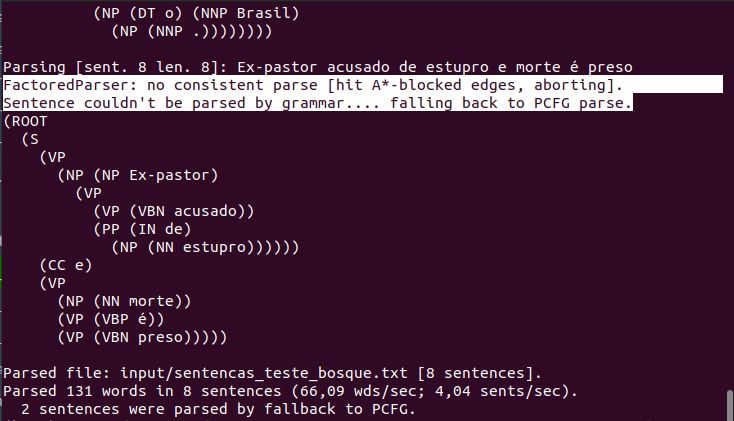
\includegraphics[width=.8\textwidth,scale=1.5]{imagens/erro_factored_parser.png}
    \caption[Erro no \textit{FactoredParser}]{Erro no \textit{FactoredParser}}
    \label{fig:bosque_erro_factored}
\end{figure}
\end{center}

\begin{center}
    \begin{figure}[!ht]
    \centering
    
    \begin{minipage}{.8\textwidth}
        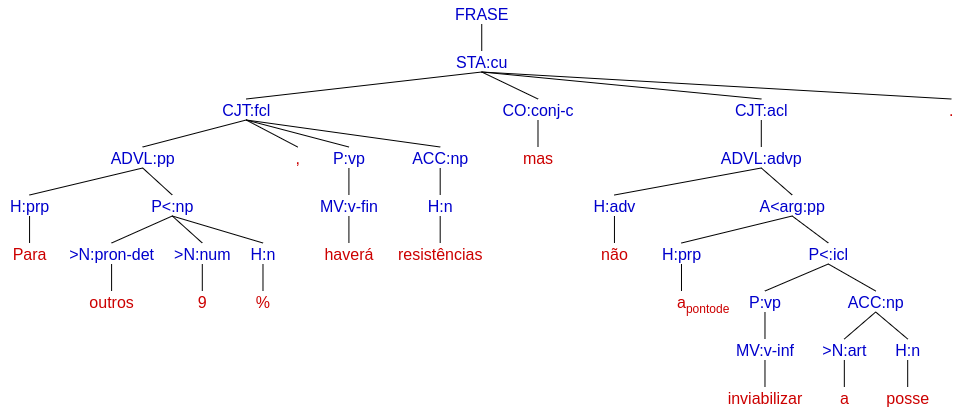
\includegraphics[width=\linewidth]{imagens/ec_bosque_perc_orig.png}
        \caption{árvore original}
    \end{minipage}
    % 
    \begin{minipage}{.8\textwidth}
        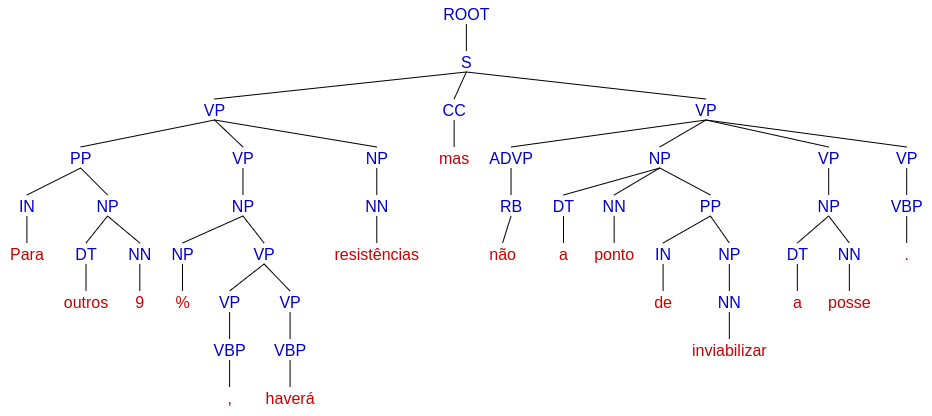
\includegraphics[width=\linewidth]{imagens/ec_bosque_perc_sp.png}
        \caption{árvore gerada pelo SP}
    \end{minipage}
    
    
    \caption[Estudo de caso BOSQUE - Sentença transduzida com sinal de porcentagem]{Estudo da sentença CF144-5, \textquote{ Para outros 9\%, haverá resistências mas não a ponto de inviabilizar a posse.}, que possui o símbolo de porcentagem. Note que, dessa vez, não há uma árvore do transdutor.}
    \label{fig:ec_bosque_perc_tree}
\end{figure}


\end{center}


\end{apendicesenv}